
%%%%%%%%%%%%%%%%% Intro %%%
\section{Introduction}
In this report the spectral analysis of irregularly sampled data - in particular line spectra - is performed using the Fourier Transform. Also, the sparse representation of signals is evaluated by applying different classical methods such as "greedy" algorithms and "convex relation" approaches. These methods are applied in particular to irregular sampled data, since this is the most realistic representation of acquired data in astronomy.


%%%%%%%%%%%%%%%%%%%% TASK II %%%%%%%%%%%%%%%%%%%%%%%%%%%
\section{Spectral analysis with Fourier Transform}
\begin{figure}[h!]
	\centering
	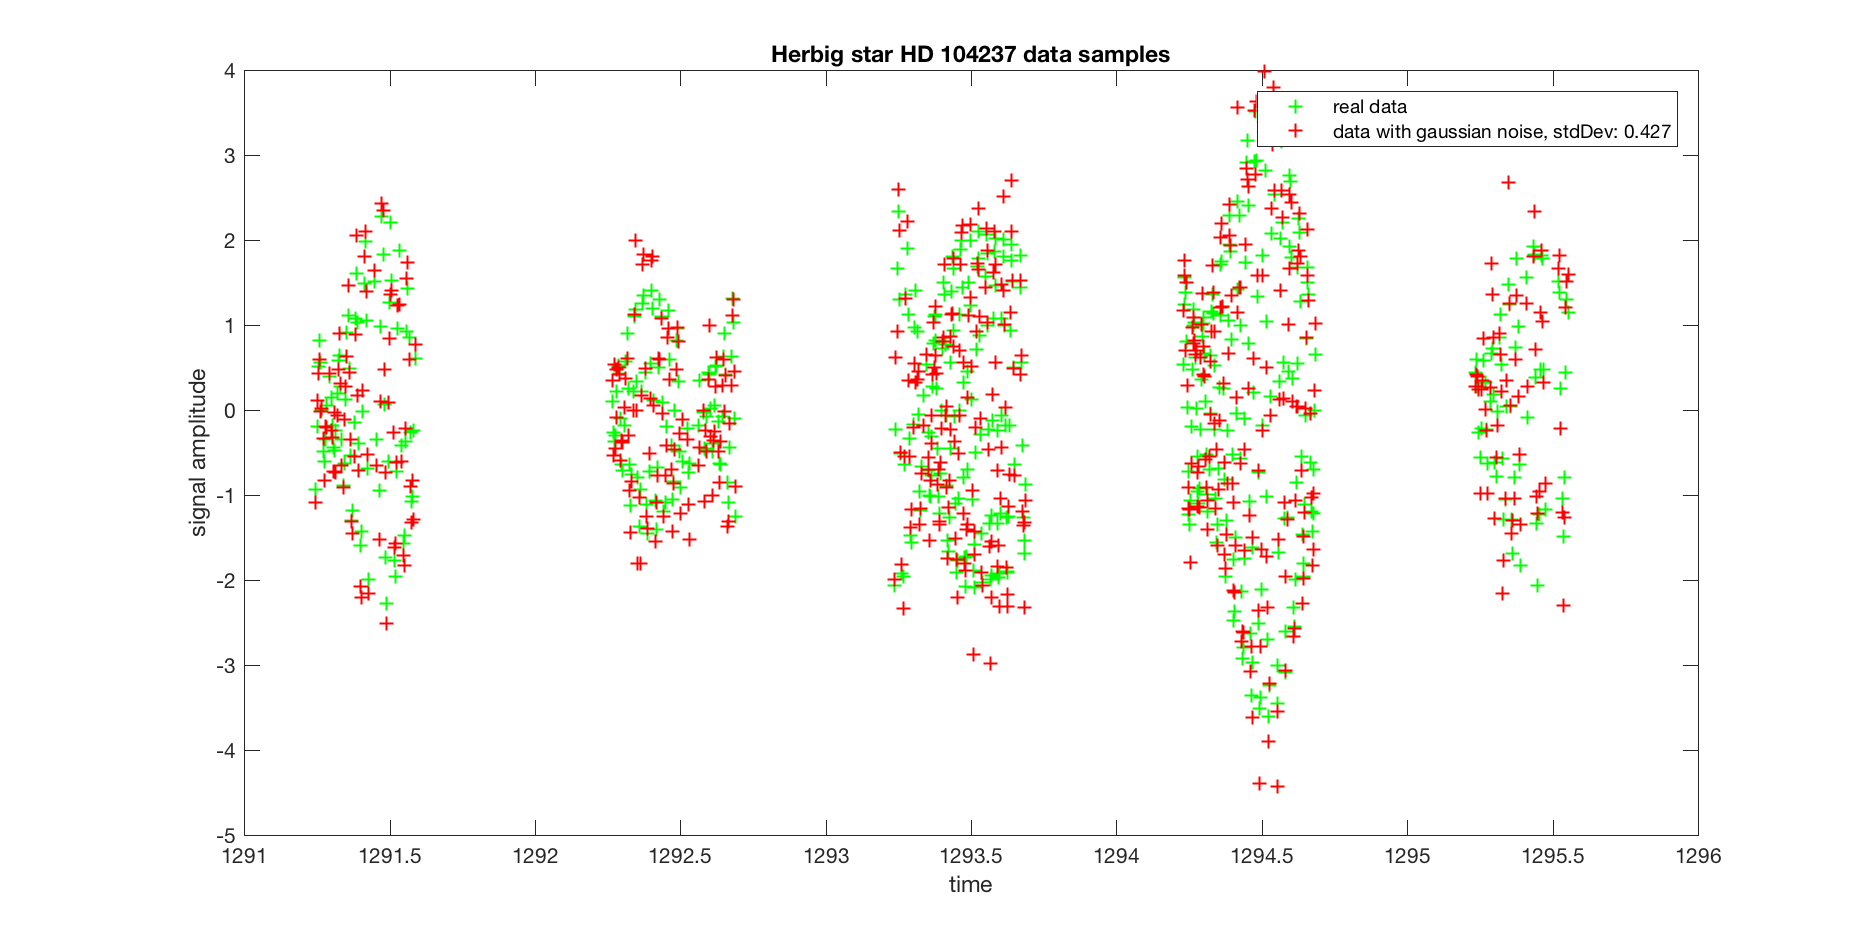
\includegraphics[width=\textwidth]{images/data}
	\caption{Original data samples and samples with additional noise in time domain}
	\label{fig:data}
\end{figure}
Since working on a real data set might be difficult, in particular when it comes to understanding the underlying techniques of the methods aforementioned, we will simulate our irregular sampled data, for which an initial dataset was given (c.f \cref{Appendix A}).
Using this amplitude, phase, time, frequency and the appropriate radial velocity data, the following formula was used to create a realistic data set that is basically a noisy sum of sine functions

\begin{equation}
	\centering
	x(t_n) = \sum_{k=1}^K A_k \sin(2\pi\nu_kt_n + \phi_k) + \epsilon_n
	\label{eq:sinesum}
\end{equation}

As for the Signal-to-Noise ratio 20dB in power mean were used, and for the number of sine functions \texttt{K = 5}, as our initial data set contained 5 different amplitudes and its according phases and frequencies (c.f. \cref{Appendix A}).
\Cref{fig:data} shows the generated data, where the green part corresponds to our simulated data without noise (hereafter seen as "real" or "original" data) and the red part including noise. The noisy data set will be used from here on in all upcoming calculations.



\subsection{Irregular sampling case}
In the case of irregular sampled data we can not apply the Fast-Fourier-Transform (FFT) as we would have in the regular case. However, the Fourier-Transform can be computed by introducing a Matrix $\boldsymbol{W}$, such as
\begin{equation}
	\centering
	\boldsymbol{W}(l,c) = \exp(2j\pi t_l f_c) \quad ,\quad \boldsymbol{\hat{x}} = \boldsymbol{W^\dagger}\boldsymbol{x}
\end{equation}
with $\boldsymbol{\hat{x}}$ being the Fourier-Transform of vector $\boldsymbol{x}$. As stated above, the FFT can not be used here, since the Matrix $\boldsymbol{W}$ must be orthogonal for the FFT - which it is not in the case of irregular sampled data.\\
Nevertheless, having this tool handy, we can now perform the Fourier Transform on irregular sampled data, e.g. on our data set represented in \cref{fig:data}.

\begin{figure}[h!]
	\centering
	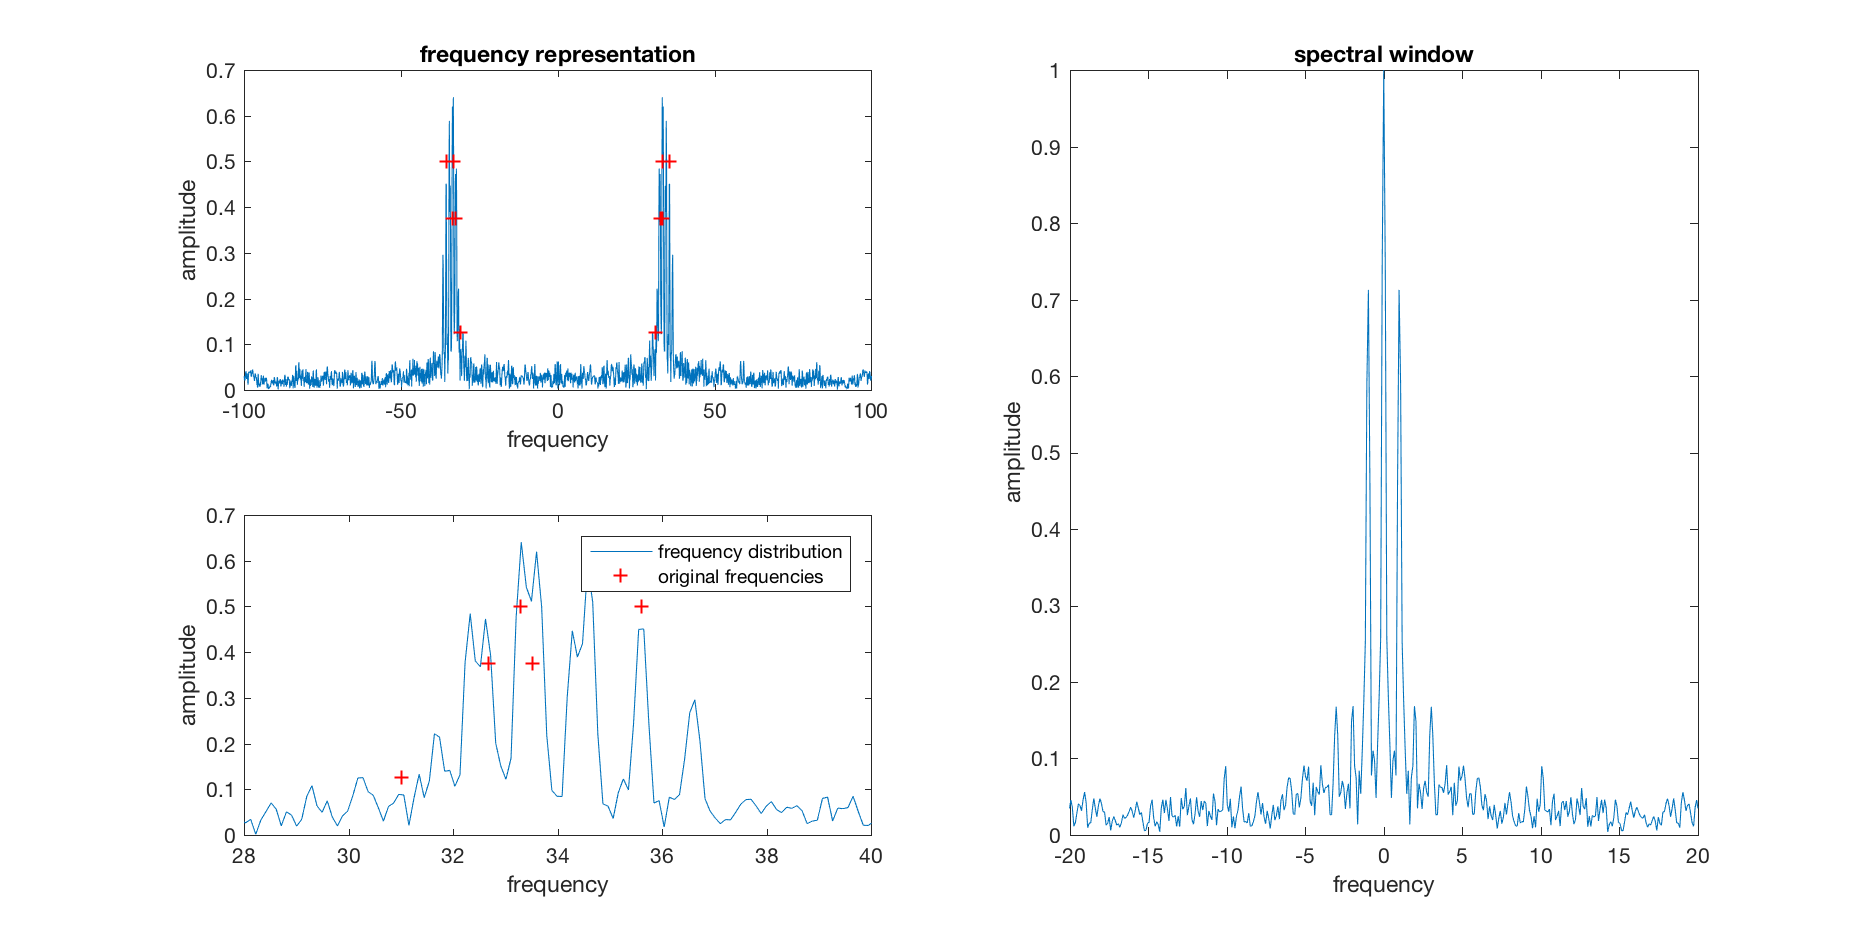
\includegraphics[width=\textwidth]{images/data_freq}
	\caption{Frequency representation with original frequencies and spectral window}
	\label{fig:data_freq}
\end{figure}

For the beginning we only use one sine-function (in \cref{eq:sinesum}, thus \texttt{K=1}). In this case it is very easy to determine the frequency and amplitude of the underlying sine-signal in the frequency representation of data, even if there are quite high side lobes. \\
\todo{can we also read out the phase from fourier diagrams?}
However, if a noisy sum of 5 sine signals is used, the underlying frequencies and amplitudes can not be easily determined anymore. This is due to the fact that the sum of signals and their noises add up, so that some peaks might be indistinguishable from others or side lobes. This can be seen in \cref{fig:data_freq} on the left side, where the red cross-hair markings correspond to the original frequency and amplitude, and the blue waveform to the frequency representation of the sum of signals. It is easy to see that the original frequencies and amplitudes can not be read out - only a rough estimation on where the frequencies might be is possible by taking into account the location of the highest peaks.

Computing the spectral window of the given frequency representation in \cref{fig:data_freq} on the left, reveals
\todo[inline]{yea, what does the spectral window tell me?}

The appropriate MATLAB code used to create the initial data set and calculate the frequency representations can be found in \cref{Appendix B}.


%%%%%%%%%%%%%%%%%%%% TASK III %%%%%%%%%%%%%%%%%%%%%%%%%%%
\section{Sparse representation with greedy algorithm}

\subsection{Pre-whitening or Matching Pursuit (MP) algorithm}




\subsection{Orthogonal Matching Pursuit (OMP) algorithm}



\subsection{Orthogonal Least Square (OLS)}



%%%%%%%%%%%%%%%%%%%% TASK IV %%%%%%%%%%%%%%%%%%%%%%%%%%%

\section{Sparse representation with convex relaxation}

